\documentclass[12pt]{article}
\usepackage{preamble}
\begin{document}
\newtheorem{assumption}{Assumption}

%%%%%%%%%%%%%%%%%frond page%%%%%%%%%%%%%%%%%%%%%%%%%%%%%%%%%%
\begin{titlepage}
\title{Counterfactual and Synthetic Control Method: Causal Inference with Instrumented Principal Component Analysis}
\author{ Cong Wang\thanks{Department of Economics and Law, Sapienza University of Rome}}
\date{\today}
\maketitle
\begin{abstract}
\noindent The fundamental problem of causal inference lies in the absence of counterfactuals. Traditional methodologies address this by implicitly or explicitly imputing the missing counterfactuals, relying on identification assumptions that are often untestable and too strong. Synthetic control methods (SCM) utilizes weighted average of control units to impute the missing counterfactual for the treated. Eventhough SCM relaxes some strict assumptions, it requires the treated unit to be inside the convex hull formulated by control units to avoid extrapolation. In recent advances, researchers modelling the entire data generating process (DGP) to impute the missing counterfactual explicitly. This paper expands the interactive fixed effect model by integrating covariates into dynamic factor loadings adding additional robustness. This methodology offers multiple benefits: firstly, it incorporates the strengths of previous SCM approaches, such as the relaxation of the untestable parallel trends assumption (PTA). Secondly, it does not require the targeted outcomes inside the convex hull formulated by control units. Thirdly, it eliminates the need for correct model specification required by interactive fixed effect (IFE) model. Finally, it inherits the ability of principal component anlaysis (PCA) to effectively handle high dimensional data and enhances the value extracted from numerous covariates.\\

\noindent\textbf{Keywords:} Synthetic Control, Principal Component Analysis, Causal Inference\\

\noindent\textbf{JEL Codes:} G11, G12, G30\\
\bigskip
\end{abstract}
\setcounter{page}{0}
\thispagestyle{empty}
\end{titlepage}
\pagebreak \newpage

\doublespacing

%%%%%%%%%%%%%%%%%%%%%%%%%%%%%%%%%%%%%%%%%%%%%%%%%%%%%%%%%%%%%%%
%%%%%%%%%%%%%%%%%%%%%%%%%%%%%%%%%%%%%%%%%%%%%%%%%%%%%%%%%%%%%%%
\section{Introduction} 
\label{sec:introduction}
%%%%%%%%%%%%%%%%%%%%%%%%%%%%%%%%%%%%%%%%%%%
In this paper, we introduce a novel counterfactual imputation method that combines the dimension reduction capabilities of principal component analysis (\cite{jollife2016principal}) with the flexibility of the interactive fixed effect model (\cite{bai2003computation,bai2009panel}). This approach not only harnesses the strengths of PCA in managing high dimensional data but also adapts the versatility of IFE to accommodate a wide range of data generating processes. We name the newly proposed method the counterfactual and synthetic control method with instrumented principal component analysis (CSC-IPCA), aligning with the previous counterfactual and synthetic control method with interactive fixed effects (CSC-IFE)\footnote{The concept of counterfactual and synthetic control (CSC) is a generalization for a group of methodolies for causal inference proposed by \cite{chernozhukov2021exact}, the original name of this methodology is actually ``generalized synthetic control method with interactive fixed effect model'' named by \cite{xu2017generalized}.} proposed by \cite{xu2017generalized}. To model the entire data generating process, the CSC-IPCA estimator is designed to overcome the constraints of untestable and stringent assumptions such as unconfoundedness and common support for matching (\cite{abadie2011bias, abadie2006large}), parallel trend assumption for diffference-in-differences (DID) (\cite{card1993minimum}), and others. Furthermore, it addresses the limitation observed in the original synthetic control method (\cite{abadie2010synthetic}) and its variants (\cite{ben2021augmented}, \cite{arkhangelsky2021synthetic}), which necessitate the outcomes of treated units to lie inside or not far from the convex hull formed by control units. 

Causal inference in economics and other social sciences is frequently complicated by the absence of counterfactuals, which is essential for evaluating the impact of a treatment or policy intervention. \cite{imbens2015causal} state that at some level, all methods for causal inference can be viewed as imputation methods, although some are more explicitly than others. For instance, under certain assumptions, the matching method (\cite{abadie2006large, abadie2011bias}) implicitly imputes the missing counterfactuals for treated units with meticulously selected control units. The DID method (\cite{card1993minimum, ashenfelter1978estimating}), on the other hand, explicitly imputes the missing counterfactuals by differencing the control units before and after treatment. While the SCM method explicitly imputes the missing counterfactual with weighted average of control units. Our method aligns with the recent trend in causal inference literature, aiming to explicitly impute the missing counterfactual by modeling the entire data generating process, a strategy highlighted by \cite{athey2021matrix} with their matrix completion (MC) method, and \cite{xu2017generalized} with their interactive fixed effect method.

Fixed effects models have long been explored in the econometrics literature related to modeling panel data, with significant contributions from \cite{bai2003computation}, \cite{pesaran2006estimation}, \cite{stock2002forecasting}, \cite{eberhardt2009cross}, among others. However, within the context of causal inference, \cite{hsiao2012panel} stands out as the first work proposing the use of this method specifically for predicting missing counterfactuals in sythetic control settings, followed by \cite{gobillon2016regional, xu2017generalized, chan2016policy} and \cite{li2018inference}. The CSC-IPCA estimator builds upon the instrumented principal component analysis first introduced by \cite{kelly2020instrumented, kelly2019characteristics} in the context of predicting stock returns. It belongs to the fixed effect method family, while through the instrumented factor loadings we can estimate the time varying latent factors more accuately. Firstly, it assumes a simple fixed effect model as with \cite{bai2003computation} with only the interactive component between factor loadings $\Lambda_i$ and time varying factors $F_t$:

\begin{equation}
\label{eqn: static}
    Y_{it} = \Lambda_i F_t + \epsilon_{it}
\end{equation}

\noindent Secondly, it instruments the factor loadings $\Lambda_i$ with covariates $X_{it}$, which allows us to capture the time varying properties of the factor loadings:

\begin{equation}
\label{eqn: instrumented}
    \Lambda_{it} = X_{it}\Gamma + H_{it}
\end{equation}

The static factor loadings $\Lambda_i$ in Equation \ref{eqn: static} are assumed to be constant by most studies in the related literature. However, in many economic and social science contexts, the factor loadings are not fixed but fluctuate over time in response to relevant covariates. This adaptation is particularly realistic in many economic and social science contexts\footnote{Considering a company that increases its investment in R\&D, it transitions from a conservative stance to a more aggressive one. This can also impact its profitability, potentially moving it from a robust position to a weaker one. The unit effect, hence, changes along with its investment strategy.}. By instrumenting the factor loadings $\Lambda_i$ with covariates $X_{it}$ through Equation \ref{eqn: instrumented}, we can capture the time varying properties of the factor loadings. The matrix $\Gamma$, serving as an $L \times K$ mapping function from covariates (number of $L$) to factor loadings (number of $K$), also acts as a dimension reduction operation, which aggregates all the information from the covariates into a smaller number of factors, making the model parsimonious.

The instrumented factor loadings enhance our estimation of the time varying latent factors $F_t$. Unlike the prediction problem addressed in \cite{kelly2020instrumented,kelly2019characteristics}, here we utilize only the control units to estimate $F_t$ and then update $\Gamma$ with the treated units before treatment. This represents the crucial distinction between our method and the IPCA method for prediction, where the mapping matrix $\Gamma$ is assumed to be constant for all units across all periods. 

This approach presents three major advantages over the CSC-IFE model and other fixed effect methods for causal inference. First, it eliminates the necessity for correct model specification, a crucial demand of the CSC-IFE method. In CSC-IFE method, aside from the interactive component $\lambda_i F_t$, the model also mandates that covariates be included in the functional form linearly as regressors $X_{it}\beta$. Second, in the CSC-IPCA method, the unit specific factor loadings $\Lambda_{it}$ are instrumented by covariates, introducing time varying characteristics to the factor loadings. This adaptation is particularly realistic in many economic and social science contexts, where unit effects are not fixed, but fluctuating over time in response to covariates. Third, the CSC-IPCA method incorporates a dimension reduction operation by matrix $\Gamma$. This step is particularly beneficial for high-dimensional datasets with a large number of covariates. This feature makes it particularly valuable for financial data (\cite{feng2020taming}) and high dimensional macroeconomic time series data (\cite{brave2009chicago}).

 






 
%%%%%%%%%%%%%%%%%%%%%%%%%%%%%%%%%%%%%%%%%%%%%%%%%%%%%%%%%%%%%%%
%%%%%%%%%%%%%%%%%%%%%%%%%%%%%%%%%%%%%%%%%%%%%%%%%%%%%%%%%%%%%%%
\section{Framework} 
\label{sec: framework}
%%%%%%%%%%%%%%%%%%%%%%%%%%%%%%%%%%%%%%%%%%%

Consider $Y_{it}$ as the observed outcome for a specific unit $i$ at time $t$. The total number of units is $N = N_{treat} + N_{\text{ctrl}}$, where $N_{treat}$ indicates the number of units in the treatment group, and $N_{\text{ctrl}}$ represents those in the control group. Each unit is observed over $T$ time periods, ranging from period 1 to period $T$. Let $T_{\text{pre}}$ denote the number of pre-treatment periods, and $T_{\text{post}}$ the number of post-treatment periods. The unit is treated at time $T_{\text{pre}} + 1$, and the treatment effect is initially observed at time $T_{\text{pre}} + 1$ and continues to be observed thereafter, a scenario commonly referred to as staggered adoption. For the data generating process of $Y_{it}$ we assume the following functinoal form:

\begin{assumption}
Functional form:
\label{ass: function}
\end{assumption}

\begin{equation}
\begin{aligned}
& Y_{it} = D_{it} \circ \delta_{it} + \Lambda_{it}F_{t} + \mu_{it}, \\
& \Lambda_{it} = X_{it}\Gamma + H_{it}
\end{aligned}
\label{eqn: functional form}
\end{equation}

\noindent where $D_{it}$ is a binary treatment indicator and $\delta_{it}$ signifies the treatment effect, which exhibits variation across units and through times\footnote{The symble ``$\circ$'' represents point-wise product.}. The expression $\Lambda_{it} = [\lambda_{it}^1, \ldots, \lambda_{it}^K]$ represents a vector of factor loadings (the number of common factors is $K$.), whereas $F_{t} = [f_{t}^1, \ldots, f_{t}^K]'$ corresponds to a vector of time-varying common factors, and $\mu_{it}$ is the idiosyncratic error term. A key distinction of the proposed model from that delineated in \cite{xu2017generalized} is the incorporation of factor loadings $B_{it}$, which are instrumented by observed covariates $X_{it}$. This integration permits $\Lambda_{it}$ to exhibit variability across time and units, thereby introducing an additional layer of heterogeneity into the model.

The vector $X_{it} = [x_{it}^1, \ldots, x_{it}^L]$ consists of observed covariates, where $L$ denotes the number of covariates. The factor loadings $\Lambda_{it}$ are assumed to be a linear function of these observed covariates $X_{it}$, with $\Gamma$ acting as the $L\times K$ coefficient matrix, and $H_{it} = [\eta_{it}^1, \ldots, \eta_{it}^L]$ comprising the vector of error terms. Another key difference from the CSC-IFE approach is that we retain only the interacted component $\Lambda_{it} F_t$ between factors and factor loadings, the linear part of covariates $X_{it}\beta$ is not included in the function form\footnote{The functional form of the CSC-IFE is $Y_{it} = D_{it} \circ \delta_{it} + \Lambda_{i}F_{t} + X_{it}\beta + \mu_{it}$}. The loagic behind is that we believe that the unit specific factor loadings, instrumented by covariates, have included all the predictive information from these covariates. This functional form allows us to handle high-dimensional datasets, especially when dealing with a large number of covariates, offering another advantage over the CSC-IFE method.

Following \cite{splawa1990application} potential outcome framework (also discussed by \cite{rubin1974estimating, rubin2005causal}), we observe the actual outcome for the treated $Y(1)$ and with the modelled data generating process we can impute the missing counterfactual $\hat{Y}(0)$. The difference between the actual outcome and imputed missing counterfactual will be the treatment effect for treated (ATT), which is defined as:

\begin{equation}
\widehat{ATT}_{t} = \frac{1}{N_{treat}}\sum_{i \in N_{treat}} \left( Y_{it}(1) - \hat{Y}_{it}(0) \right) = \frac{1}{N_{treat}}\sum_{i \in N_{treat}}\hat{\delta}_{it}.
\end{equation}
%%%%%%%%%%%%%%%%%%%%%%%%%%%%%%%%%%%%%%%%%%%%%%%%%%%%%%%%%%%%%%%
\subsection{Assumptions for identification}

\begin{assumption}
Unconfoundedness:
\label{ass: unconfoundedess} 
\end{assumption}

\begin{equation}
\epsilon_{it} \perp D_{js}, X_{js}, F_s \quad \forall i, j, s, t.
\label{eq: unconfoundedess}
\end{equation}

Assumption \ref{ass: unconfoundedess} stipulates that the error term for any unit at any time period is independent of treatment assignment, observed covariates, and unobserved time-varying factors. This independence is a crucial condition that lends substance to model Equation \ref{eq: combined} and is imperative for the consistent estimation of $\Gamma$.

\begin{assumption}
Regularity conditions: (1) $\Gamma$ is bounded and has a finite second moment, (2) $F_t$ is bounded and has a finite second moment, (3) $X_{it}$ is bounded and has a finite second moment.
\label{ass: regularity}
\end{assumption}

The regularity conditions outlined in Assumption \ref{ass: regularity} are essential for the consistent estimation of $\Gamma$ and $F_{t}$. Specifically, these conditions ensure that the matrix $\Gamma'X'_tX_t\Gamma$, which is involved in inversion processes, remains nonsingular (where $X_t$ denotes the $N \times L$ matrix consisting of the cross-section of $x_{i,t}$).

\begin{assumption}
Asymptotic normality:
\begin{enumerate}
\renewcommand*\labelenumi{(\theenumi)}
\item $\text{As } N, T \to \infty, \: \frac{1}{\sqrt{NT}} \sum_{i,t} \text{vect}\left( X'_{i,t} \epsilon_{i,t} F'_{t} \right) \xrightarrow{d} \text{Normal} \left(0, \Omega^{x\epsilon f} \right)$,
\item $\text{As } N \to \infty, \: \frac{1}{\sqrt{N}} \sum_{i} \text{vect}\left( X'_{i} \epsilon_{i} \right) \xrightarrow{d} \text{Normal} \left(0, \Omega^{x\epsilon} \right) \: \text{for} \: \forall t$,
\item $\text{As } N, T \to \infty, \: \frac{1}{\sqrt{T}} \sum_{t} \text{vect}\left( F_{t}F'_{t} - E[F_{t}F'_{t}] \right) \xrightarrow{d} \text{Normal} \left(0, \Omega^{f} \right)$.
\end{enumerate}
\label{ass: asy normal}
\end{assumption}

Assumption \ref{ass: asy normal} simply containes central limit theorems with respect to different variables, which are satisfied by various mixing processes.

%%%%%%%%%%%%%%%%%%%%%%%%%%%%%%%%%%%%%%%%%%%%%%%%%%%%%%%%%%%%%%%
%%%%%%%%%%%%%%%%%%%%%%%%%%%%%%%%%%%%%%%%%%%%%%%%%%%%%%%%%%%%%%%
\section{Estimation}
\label{sec: estimation}
%%%%%%%%%%%%%%%%%%%%%%%%%%%%%%%%%%%%%%%%%%%%%%%%%%%
The CSC-IPCA estimator of the treatment effect for a treated unit $i$ at time $t$ is defined as the difference between the observed outcome and its estimated counterfactual: $\delta_{it} = Y_{it}(1) - \hat{Y}_{it}(0)$. To combine the functional form in Equation \ref{eqn: functional form}, we get the structural component of the potential outcome $Y_{it} = (X_{it}\Gamma) F_{t}$. The CSC-IPCA method is estimated by minimizing the sum of squared residuals of the following objective function:

\begin{equation}
\label{eqn: obj}
\underset{\Gamma, F_t}{\arg\min} \sum_{i} \sum_{t}\left( Y_{it} - (X_{it}\Gamma) F_{t} \right)^2.
\end{equation}

Unlike the IFE method (\cite{bai2009panel}), our approach requires estimating only two parameters, $\Gamma$ and $F_t$, simplifying the process. Different from principal component analysis (\cite{jolliffe2002principal}), our method involves using covariates to instrument the factor loadings component. This necessitates the estimation of $\Gamma$ rather than $\Lambda_i$, so we can not directly use eigenvalue decomposition. While the objective function in Equation \ref{eqn: obj} formulates the problem as minimizing a quadratic function with a single unknown variable (e.g., $\Gamma$) while holding the other variable (e.g., $F_t$) constant. This structure enables the application of the alternating least squares (ALS) method for a numerical solution. Generally, the imputation for the missing counterfactual $Y_{it}(0)$ is executed in three steps:

\textbf{Step 1:} The initial step entails estimating the time-varying factors $\hat{F}_t$ and the coefficient matrix $\hat{\Gamma}_{\text{ctrl}}$ utilizing an ALS algorithm, based exclusively on data from the control group for the whole time period.

\begin{equation}
(\hat{\Gamma}_{ctrl}, \hat{F_t}) = \underset{\Gamma, F_t}{\arg\min} \sum_{i \in N_{ctrl}} \sum_{t \in T}\left( Y_{it} - (X_{it}\Gamma) F_{t} \right)'\left( Y_{it} - (X_{it}\Gamma) F_{t} \right).
\tag{3}
\label{eq: optimization}
\end{equation}

\textbf{Step 2:} The subsequent step involves estimating the coefficient matrix $\hat{\Gamma}_{treat}$ for treated unit $i$ at time $t$, employing the previously estimated time-varying factors $\hat{F}_t$ and the observed covariates $X_{it}$, using only pretreatment data from the treated units.

\begin{equation}
\hat{\Gamma}_{treat} = \underset{\Gamma}{\arg\min} \sum_{i \in N_{treat}} \sum_{t \in T_{pre}} \left( Y_{it} - (X_{it} \Gamma) \hat{F}_{t} \right)' \left( Y_{it} - (X_{it} \Gamma) \hat{F}_{t} \right).
\tag{4}
\end{equation}

\textbf{Step 3:} The final step involves imputing the counterfactual outcome $\hat{Y}_{it}(0)$ for treated unit $i$ at time $t$ by substituting the estimated coefficient matrix $\hat{\Gamma}_{treat}$ and the time-varying factors $\hat{F}_t$ into the following equation:

\begin{equation}
\hat{Y}_{it}(0) = (X_{it} \hat{\Gamma}_{treat}) \hat{F}_{t}, \quad \forall i \in N_{treat}, \forall t \in T_{post}.
\tag{5}
\end{equation}

The main difference between CSC-IPCA and the instrumented principal component analysis (IPCA) as proposed by \cite{kelly2020instrumented} lies in the purpose of prediction. In the IPCA method, the authors predict the next-period stock returns using all covariates from the preceding period, under the assumption that the rotation matrix $\Gamma$ remains constant across all observations. In contrast, CSC-IPCA introduces a pivotal distinction: it operates under the assumption that treated and control groups are characterized by unique rotation matrices, $\Gamma_{\text{treat}}$ and $\Gamma_{\text{ctrl}}$. This assumption is vital for the unbiased estimation of the ATT, setting the CSC-IPCA method apart by directly addressing heterogeneity in the treatment effect through the specification of group-specific rotation matrices.

\subsection{Hyper parameter tuning}
%%%%%%%%%%%%%%%%%%%%%%%%%%%%%%%%%%%%%%%%%%%%%%%%%%%
Similar to CSC-IFE methods, researchers often encounter the challenge of selecting the appropriate number of factors, $K$, without prior knowledge of the true data-generating process. To facilitate this selection, we introduce data-driven approaches for determining the hyperparameter $K$. Utilizing both control and treated units as training and validation data respectively offers a practical solution. To enhance the robustness of this process, we propose two validation methods for hyperparameter tuning. Algorithm \ref{algorithm: 1} describes a bootstrap method to ascertain $K$. This approach involves repeatedly sampling $N_{ctrl}$ control units for training data and $N_{treat}$ treated units for validation data, both with replacement. The optimal $K$ is then determined by minimizing the average of sum squared errors across these validations.

\begin{algorithm}[!ht]
    \SetAlgoLined
    \KwData{$Y, X$}
    \KwResult{Optimal hyperparameter $k$}
    Determine the maximum possible hyperparameter $K$ and the number of repetitions $N$\;

    Initialize an array $MSE$ to store the average of sum squared error for each $k$\;
    \For{$k \leftarrow 1$ \KwTo $K$}{
        Initialize sum of squared errors: $SSE_k \leftarrow 0$\;
        \For{$n \leftarrow 1$ \KwTo $N$}{
            Construct a bootstrap training dataset $(Y^{b}_{ctrl}, X^{b}_{ctrl})$ by sampling $N_{ctrl}$ control observations with replacement\;

            Construct a bootstrap validation dataset $(Y^{b}_{treat}, X^{b}_{treat})$ by sampling $N_{treat}$ treated observations with replacement\;

            Estimate parameters $\Gamma$ and $F_t$ using the training data via the ALS method\;

            Use the estimated $\hat{\Gamma}$ and $\hat{F}_t$ to predict $\hat{Y}^{b}_{treat}$ with the validation data\;

            Compute the sum of squared error for the validation data: $SE_n \leftarrow \sum\left(Y^{b}_{treat} - \hat{Y}^{b}_{treat}\right)^2$\;

            Accumulate the sum of squared errors: $SSE_k \leftarrow SSE_k + SE_n$\;
        }
        Calculate the average sum squared error for $k$: $MSE[k] \leftarrow \frac{SSE_k}{N}$\;
    }
    Select $k$ corresponding to the minimum value in $MSE$\;
    \caption{Bootstrap Hyperparameter Tuning}
    \label{algorithm: 1}
\end{algorithm}

We can also utilize leave-one-out cross-validation to select the hyperparameter $K$, as detailed in Algorithm 2. This method involves excluding the $t^{th}$ period data from the control group to serve as the training data, while similarly excluding the corresponding period data from the treated group to act as validation data. This process is repeated for each time period in the pretreatment phase, applying a predetermined number of factor loadings. The optimal number of factors, $K$, is identified as the one that yields the minimum average of sum squared errors across all iterations.

\begin{algorithm}[!ht]
    \SetAlgoLined
    \KwData{$Y, X$}
    \KwResult{Optimal hyperparameter $k$}
    Determine the maximum possible hyperparameter $K$\;
    Initialize an array $MSE$ to store the average of sum squared error for each $k$\;
     \For{$k=1$ to $K$}{
        Set sum of squared errors $SSE_k = 0$\;
        \For{$t \leftarrow 1$ to $T_{pre}$}{
            Remove the $t^{th}$ period observation from control data, using the rest as training data $(Y_{ctrl}^{-t}, X_{ctrl}^{-t})$\;
            
            Similarly, exclude the $t^{th}$ period observation from treated data, using the rest as validation data $(Y_{treat}^{-t}, X_{treat}^{-t})$\;
            
            Estimate parameters $\Gamma$ and $F_t$ using the training data via the ALS method\;
            
            Use the estimated $\hat{\Gamma}$ and $\hat{F}_t$ to predict $\hat{Y}^{-t}_{treat}$ with the validation data\;
            
            Calculate the sum squared error $SE_t = \sum (Y_{treat}^{-t} - \hat{Y}_{treat}^{-t})^2$\;
            
            Accumulate the sum of squared errors:  $SSE_k \leftarrow SSE_k + SE_t$\;
        }
        Calculate the average sum squared error for $k$: $MSE[k] = \frac{SSE_k}{T_{pre}}$\;
      }
      Select $k$ corresponding to the minimum value in $MSE$\;
    \caption{Leave-One-Out Cross-Validation for Hyperparameter $k$}
    \label{algorithm: 2}
\end{algorithm}

\subsection{Inference}
%%%%%%%%%%%%%%%%%%%%%%%%%%%%%%%%%%%%%%%%%%%%%%%%%%%

In the context of causal inference, the pioneering application of the interactive fixed effect model is attributed to \cite{hsiao2012panel}. Nonetheless, a formal framework for inference using this method was not established until the works of \cite{chan2016policy} and \cite{li2018inference}. These methods of inference rely on a large number of control units and pre treatment periods to develop asymptotic properties. In recent years, conformal inference (\cite{chernozhukov2021exact}) has gained popularity in causal inference literature, such as \cite{ben2021augmented}, \cite{roth2023s}, and \cite{imbens2024causal}. Conformal inference is a nonparametric method that provides and exact and robust inference without requiring the specification of a model. Our causal inference framework, designed for predicting missing counterfactuals, allows us to construct inference procedures based on conformal prediction introduced by \cite{shafer2008tutorial} for the robustness against misspecification. The causal effect is identified as the difference between the observed outcomes and these estimated counterfactuals, expressed mathematically as:

\begin{equation*}
\theta_{it} = Y_{it} - \hat{Y}_{it}, \quad \forall i \in N_{tr}, \quad \text{and} \quad \forall t \in T_{post},
\end{equation*}

\noindent where $\theta_{it}$ denotes the treatment effect for unit $i$ at time $t$, and $\hat{Y}_{it}$ represents the imputed counterfactual outcome. 
    
To conduct conformal inference, we first postulate a sharp null hypothesis, $H_0: \theta_{it} = \theta_{it}^0$. Under this null hypothesis, we adjust the outcome for treated units post treatment as $\tilde{Y}_{it} = Y_{it} - \theta_{it}$. We then replace the original dataset with this adjusted part, $\tilde{Y}_{it}$. Secondly, following the estimation procedures described in Section \ref{sec: estimation} to estimate the time varying factor $F$ with only control data as before, and update the $\Gamma$ for the newly adjusted treated units with the entire set of treated units\footnote{As a clarification, in the estimation section, we update $\Gamma$ using only the treated units before treatment. However, for inference, we use the entire set of treated units to update 
$\Gamma$.}. The concept revolves around updating the $\Gamma$ using all the treated units, under the assumed null hypothesis, to minimize the occurrence of large residuals after intervention.

Thirdly, we estimate the treatment effect and compute the residuals for the treated units in the post treatment period. The test statistic showing how large the residual is under the null:

\begin{equation}
S(\hat{\mu}) = \left(\frac{1}{\sqrt{T_*}}\sum_{t \in T_1} |\hat{\mu}|^q \right)
\end{equation}

Where $\hat{\mu}$ represents the residual for the treated units in the post-treatment periods, we employ $q=1$ for the permanent intervention effect as designed in our study. A high value of the test statistic indicates a poor post treatment fit, suggesting that the treatment effect postulated by the null is unlikely to be observed, hence leading to the null's rejection. 

Finally, we block permute the residuals and calculate the test statistic in each permutation. The P-value is defined as:
\begin{equation}
\hat{p} = 1 - \hat{F}(S(\hat{u})), \text{ where } \hat{F}(x) = \frac{1}{|\Pi|} \sum_{\pi \in \Pi} 1\{S(\hat{u}_\pi) < x\}.
\end{equation}

\noindent where $\Pi$ represents the set of all block permutations, the test statistic for each permutation is denoted by $S(\hat{\mu}_{\pi})$, , with $x$ being the test statistic calculated from the unpermuted residuals. By employing different sets of nulls, we can compute a confidence interval at a specified confidence level.

%%%%%%%%%%%%%%%%%%%%%%%%%%%%%%%%%%%%%%%%%%%%%%%%%%%%%%%%%%%%%%%
%%%%%%%%%%%%%%%%%%%%%%%%%%%%%%%%%%%%%%%%%%%%%%%%%%%%%%%%%%%%%%%
\section{Monte Carlo Simulation}
\label{sec: simulation}
%%%%%%%%%%%%%%%%%%%%%%%%%%%%%%%%%%%%%%%%%%%%%%%%%%%

In this section, we employ Monte Carlo simulations to assess the performance of the CSC-IPCA estimator in finite sample settings. We juxtapose the CSC-IPCA estimator against the CSC-IFE and the original SC estimators. Our comparative analysis focuses on key metrics including bias, mean squared errors, and coverage probability. 

We initiate our analysis with a data generating process that incorporates $L=10$ and $K=3$ time-varying covariates and common factors, along with unit and time fixed effects:

\begin{equation}
Y_{it} = D_{i} \delta_{t} + X_{it}\beta + (X_{it}\Gamma) F_{t} + \alpha_i + \xi_t + \epsilon_{it}.
\tag{6}
\label{eq: dgp}
\end{equation}

\noindent where $X_{it} = [x_{it}^1, \ldots, x_{it}^{L}]$ denotes a vector of $L \times 1$ time-varying covariates, which follows a VAR(1) process. $X_{it} = \mu_i + A_i X_{i,t-1} + \nu_{it}$, where $A_i$ is a $ L \times L$ variance-covariance matrix\footnote{In our methodology, the variance-covariance matrix is not constrained to be diagonal, thus allowing covariates within each unit to be correlated, reflecting the typical scenario in most economic time series data. To emphasize the independence among different units, we generate $N$ unique variance-covariance matrices, each corresponding to a unit, ensuring cross-sectional independence and preserving time-series correlation. Moreover, we impose a condition on these matrices by requiring the eigenvalues of $A_i$ to have characteristic roots that reside inside the unit circle, thereby assuring the stationarity of the VAR(1) process.}, The drift term $\mu_i$ equals 0 for control units and 2 for treated units,\footnote{This configuration underscores that the treatment assignment is not random; rather, it depends on the covariates $X_{it}$.}, and $\nu_{it}$ is a $L \times 1$ vector of i.i.d. standard normal errors. While $F_t = [f_t^1, \ldots, f_t^3]^\prime$ denotes the vector of time-varying common factors, adhering to a similar VAR(1) process, the variable $\epsilon_{it}$ represents the idiosyncratic error term. Unit and time fixed effects, $\alpha_i$ and $\xi_{t}$ respectively, are uniformly drawn from the interval $(0,1)$. The coefficient vector $\beta = [\beta^1, \ldots, \beta^{L}]^\prime$ associated with the covariates is drawn uniformly from $(0,1)$, and $\Gamma$, the $L \times K$ coefficient matrix for the factor loadings, is drawn uniformly from $(-0.1, 0.1)$, with these covariates serving as instruments. The treatment indicator $D_{it}$ is binary, defined as $D_{it} = 1$ for treated units during post-treatment periods, and $D_{it} = 0$ otherwise. The heterogeneous treatment effect is modeled as $\delta_{it} = \bar{\delta}_{it} + e_{it}$, where $e_{it}$ is i.i.d as standard normal, and $\bar{\delta_t} = [0, \cdots, 0, 1,2,\ldots,T_{post}]$ represents a time-varying treatment effect\footnote{Here we simplify the treatment effect to be constant across units, however the heterogeneous treatment effect across units can also be easily employed.}. Only the outcome $Y_{it}$, the covariates $X_{it}$, and the treatment indicator $D_{it}$ are observed, while all other variables remain unobserved.

\begin{figure}[!ht]
    \centering
    \caption{\textbf{CSC-IPCA Data Generating Process}}
    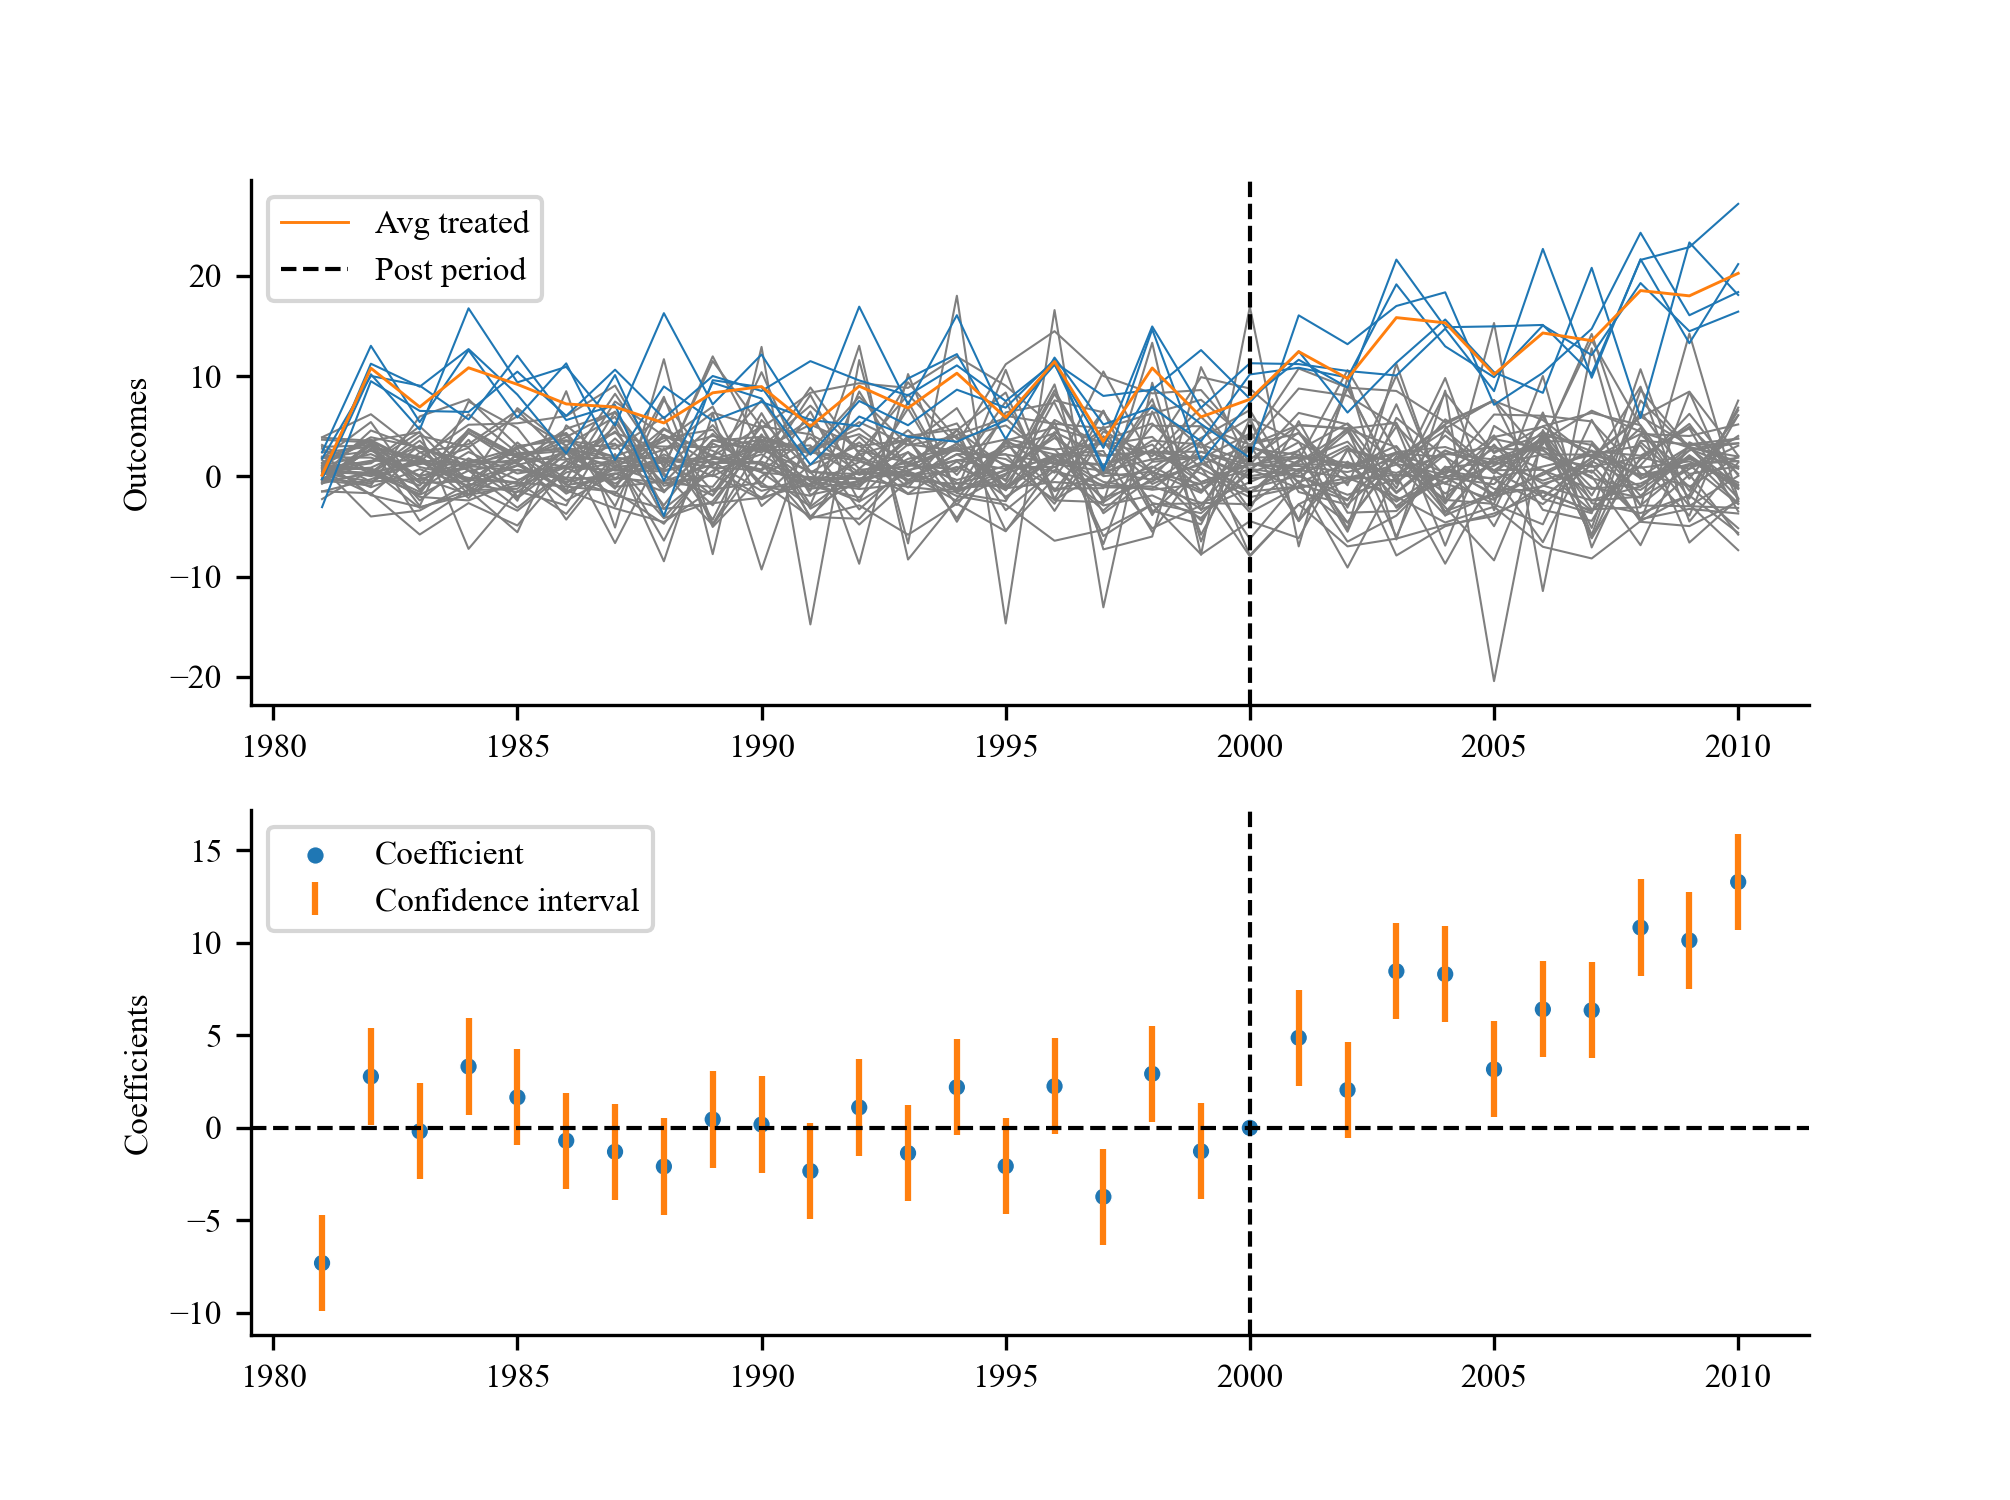
\includegraphics{figs/data_plot.png}
    \label{fig: sim}
    \caption*{\footnotesize{In this graphic, the upper panel plots simulated data following the above data generating process. The light blue lines represent treated units and the light gray lines represent controls. Key parameters are$N_{treat} = 5, N_{ctrl} = 45, T_0=20, T_1=10, L=10$. The lower panel plots a simple event study.}}
    \end{figure}

Figure \ref{fig: sim} represents the simulated data following our data generating process. Observations from the upper panel indicate that the parallel trend assumption is not met. To verify this, we plot a simple event study, clearly revealing a failure in the parallel trend assumption. Furthermore, outcomes for treated units are marginally higher than for control units. In such cases, the synthetic control method will be biased, as it avoids extrapolation and typically fit poorly for treated units.

\subsection{A simulated example}
Following this data generating process, figure \ref{fig: est} illustrates both the raw data and the imputed counterfactual outcomes as estimated by the CSC-IPCA method. In the upper panel, control units are represented in gray and treated units in light blue, with the average outcome for treated units highlighted in orange. The imputed synthetic average for treated outcomes is also shown, delineated by an orange dashed line. The CSC-IPCA method is capable of capturing the trajectory of the average outcome for treated units before treatement. The lower panel of Figure \ref{fig: est} shows the estimated ATT (dashed line) with the true ATT (solid line). The CSC-IPCA method is able to capture the true ATT, as evidenced by the close alignment between the dashed and solid lines.

\begin{figure}[!ht]
    \centering
    \caption{\textbf{CSC-IPCA Estimated ATT for Simulated Sample}}
    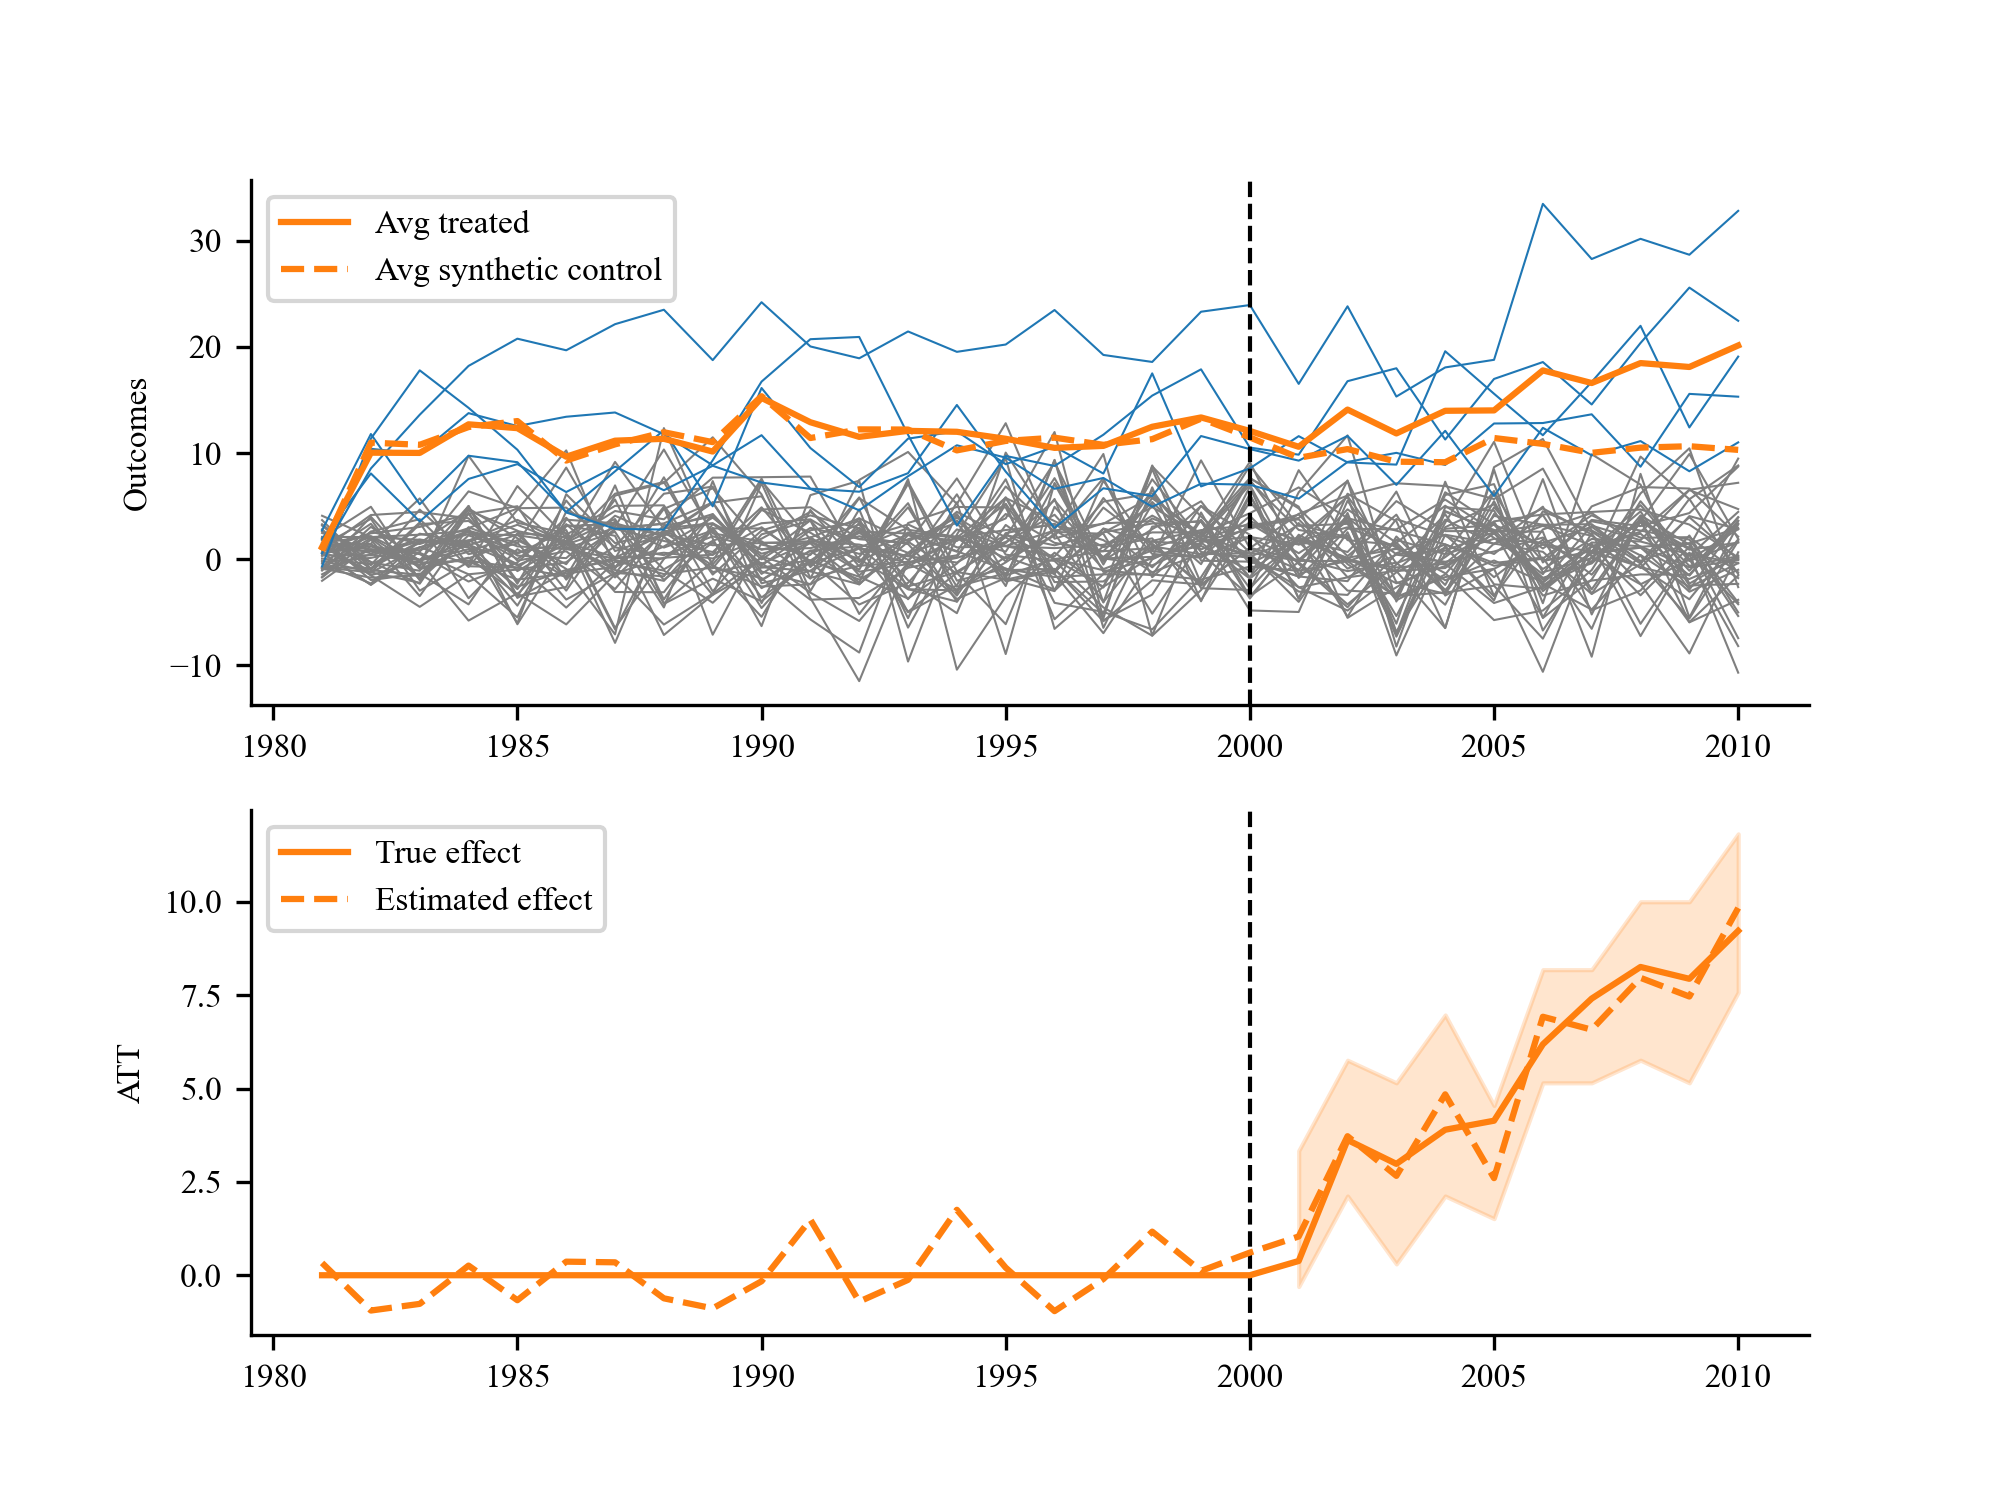
\includegraphics{figs/estimation.png}
    \label{fig: est}
    \caption*{\footnotesize{This graphic plots the CSC-IPCA method estimated ATT for simulated data $N_{treat} = 5, N_{ctrl} = 45, T_0=20, T_1=10, L=10$.}}
    \end{figure}

\subsection{Bias comparision}
Based on the same data generating process and parameters, we compare the CSC-IPCA, CSC-IFE, and SCM estimators with 1000 simulations. Figure \ref{fig: bias} illustrates the bias among these estimation methods. In panel 1, where all covariates are observed, both CSC-IPCA and CSC-IFE demonstrate unbiasedness and effectively estimate the true ATT. However, due to the outcomes of treated units falling outside the convex hull of control units, the SCM exhibits an upward bias. This scenario is common in empirical studies where only a limited number of covariates are observed. As depicted in Figure \ref{fig: bias}, from left to right, we progressively observe all 10, then 6 (2/3), and finally 3 (1/3) covariates. With an increase in the number of unobserved covariates, both CSC-IPCA and CSC-IFE lose efficiency; however, the CSC-IPCA estimator remains unbiased.

\begin{figure}[!ht]
\centering
\caption{\textbf{Bias Comparing with Other Methods}}
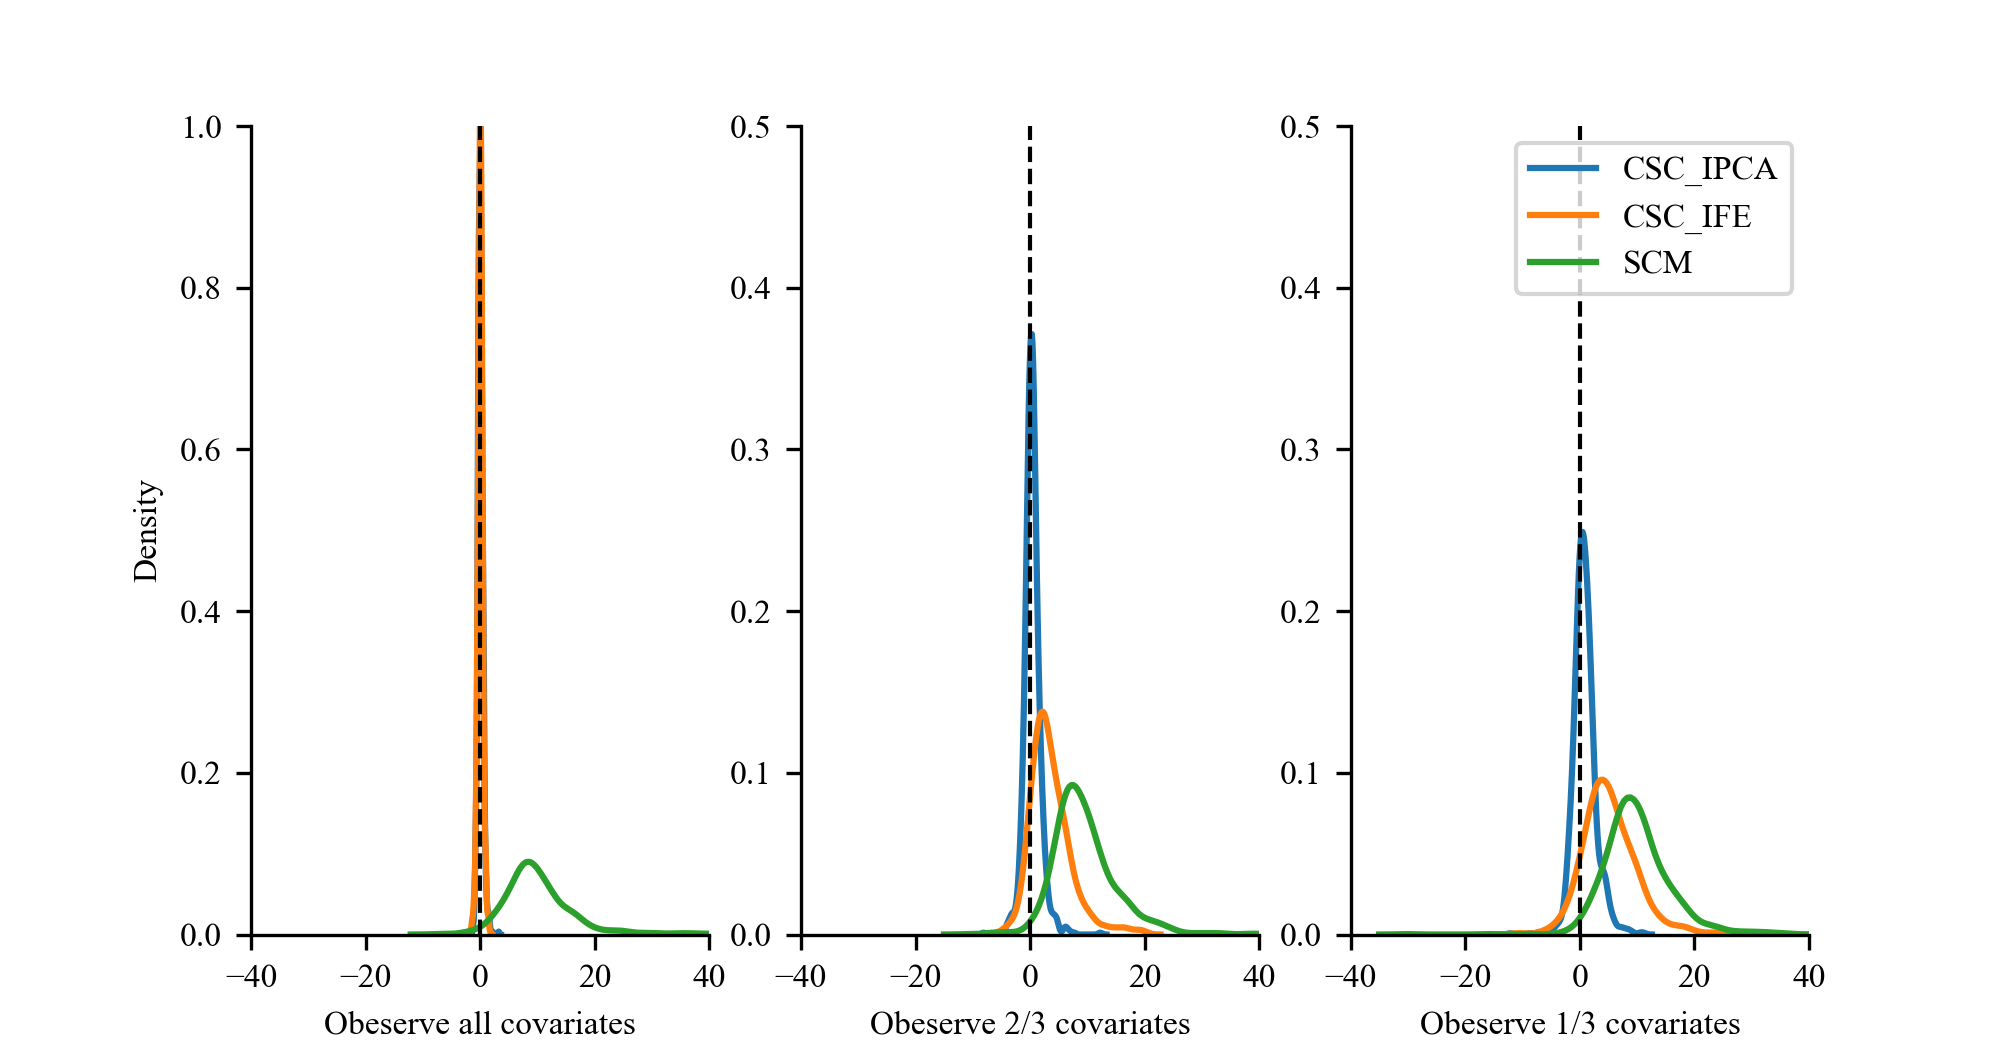
\includegraphics{figs/bias_compar1.png}
\label{fig: bias}
\caption*{\footnotesize{This graphic plots the CSC-IPCA method estimated ATT for simulated data $N_{treat} = 5, N_{ctrl} = 45, T_0=20, T_1=10, L=10$.}}
\end{figure}

\subsection{Finate sample properties}
We present the Monte Carlo simulation results in Table \ref{tab: finate sample} to investigate the finate sample properties of the CSC-IPCA estimator. The number of treated units and post treatment period are fixed to $N_{treat} = 5, T_1=5$. We vary the number of control units $N_{co}$, pre treatment period $T_0$ , and the proportion of observed covariates $\alpha$ with the total number of covariates $L=10$ to investigate the finate sample properties. As showing in the table \ref{tab: finate sample}, the bias, RMSE, and STD are estimated based on 1000 simulations\footnote{The root mean squared error (RMSE) is defined as $RMSE = \sqrt{\frac{1}{T_1}\sum_{t \in T_1}\left(ATT_t - \widehat{ATT}_t\right)^2}$. The standard deviation (STD) is defined as $STD = \frac{1}{T_1}\sum_{t \in T_1}\left(\widehat{ATT}_t - \frac{1}{T_1}\sum_{t \in T_1}\widehat{ATT_t}\right)^2$}. The results indicate that the bias of the CSC-IPCA estimator decreases as the number of control units and pre treatment period increases. The bias decreases the most when the proportion of observed covariates increases from $\frac{1}{3}$ to 1 (all covariates are observed). We observe similar pattern in RMSE and STD. It is worth noting that if we observe all the covariates (i.e., $\alpha = 1$), the bias, RMSE, and STD of the CSC-IPCA estimator are all reduce to the lowest level even with a small number of control units and pre treatment period.

\begin{table}[!ht]
\centering
\caption{\textbf{Finate Sample Properties}}
\label{tab: finate sample}
\begin{tabular}{cc|ccc|ccc|ccc}
\toprule
\multicolumn{2}{c|}{$\alpha$} & $\frac{1}{3}$ & $\frac{2}{3}$ & 1 & $\frac{1}{3}$ & $\frac{2}{3}$ & 1 & $\frac{1}{3}$ & $\frac{2}{3}$ & 1 \\
\hline
$T_0$ & $N_{co}$ & \multicolumn{3}{c|}{Bias} & \multicolumn{3}{c|}{RMSE}  & \multicolumn{3}{c}{STD} \\
\hline
10 & 10 & 2.382 & 0.747 & 0.189 & 4.619 & 3.011 & 1.712 & 3.975 & 2.943 & 1.732 \\
10 & 20 & 1.452 & 0.420 & 0.063 & 3.538 & 2.180 & 0.984 & 3.273 & 2.186 & 1.076 \\
10 & 40 & 0.920 & 0.222 & 0.008 & 2.747 & 1.745 & 0.789 & 2.650 & 1.786 & 0.917 \\
\cline{1-11}
20 & 10 & 2.534 & 1.121 & 0.237 & 4.441 & 3.015 & 1.192 & 3.688 & 2.829 & 1.271 \\
20 & 20 & 1.520 & 0.421 & 0.048 & 3.276 & 1.840 & 0.872 & 2.946 & 1.849 & 0.977 \\
20 & 40 & 1.008 & 0.258 & 0.036 & 2.632 & 1.451 & 0.539 & 2.498 & 1.505 & 0.705 \\
\cline{1-11}
40 & 10 & 2.746 & 1.148 & 0.227 & 4.982 & 2.863 & 1.167 & 4.166 & 2.665 & 1.201 \\
40 & 20 & 1.733 & 0.540 & 0.089 & 3.964 & 1.783 & 0.732 & 3.607 & 1.757 & 0.874 \\
40 & 40 & 0.807 & 0.281 & 0.044 & 2.530 & 1.632 & 0.531 & 2.457 & 1.654 & 0.677 \\
\bottomrule
\end{tabular}
\begin{tablenotes}
    \item This table presents the finate sample properties of the CSC-IPCA method estimated ATT for simulated data. The number of treated units and post treatment period are fixed to $N_{treat} = 5, T_1=5$. We vary the number of control units $N_{co}$, pre treatment period $T_0$, and proportion of observed covariates $\alpha$ to investigate the finate sample properties, the total number of covariates is $L=10$. The bias, RMSE, and STD are estimated based on 1000 simulations.
\end{tablenotes}
\end{table}
%%%%%%%%%%%%%%%%%%%%%%%%%%%%%%%%%%%%%%%%%%%%%%%%%%%%%%%%%%%%%%%
%%%%%%%%%%%%%%%%%%%%%%%%%%%%%%%%%%%%%%%%%%%%%%%%%%%%%%%%%%%%%%%
\section{Empirical Application}
\label{sec: application}
%%%%%%%%%%%%%%%%%%%%%%%%%%%%%%%%%%%%%%%%%%%%%%%%%%%

In this section, we study the CSC-IPCA method with an empirical example. We apply the CSC-IPCA method to estimate the treatment effect of the Job Corps program on the earnings of participants. The Job Corps program is a federally funded education and vocational training program for disadvantaged youth in the United States. The program provides free education and vocational training to young people aged 16 to 24, with the aim of improving their employment prospects. The program has been evaluated in several studies. The data used in this study is from the National Job Corps Study (NJCS), which is a large-scale randomized controlled trial conducted in the 1990s. The NJCS data includes a sample of 16,000 young people who were randomly assigned to either the Job Corps program or a control group. The data includes information on the participants' earnings, education, and employment history. The data also includes a rich set of covari
%%%%%%%%%%%%%%%%%%%%%%%%%%%%%%%%%%%%%%%%%%%%%%%%%%%%%%%%%%%%%%%
%%%%%%%%%%%%%%%%%%%%%%%%%%%%%%%%%%%%%%%%%%%%%%%%%%%%%%%%%%%%%%%
\section{Conclusion} 
\label{sec: conclusion}
%%%%%%%%%%%%%%%%%%%%%%%%%%%%%%%%%%%%%%%%%%%%%%%%%%%%%%%

Firms' 

\clearpage
%%%%%%%%%%%%%%%%%%%%%%%%%%%%%%%%%%%%%%%%%%%%%%%%%%%%%%%%%%%%%%%
%%%%%%%%%%%%%%%%%%%%%%%%%%%%%%%%%%%%%%%%%%%%%%%%%%%%%%%%%%%%%%%
\begingroup
\setstretch{1.0}
\bibliographystyle{plainnat}
\bibliography{citation}
\endgroup

\clearpage
%%%%%%%%%%%%%%%%%%%%%%%%%%%%%%%%%%%%%%%%%%%%%%%%%%%%%%%%%%%%%%%
%%%%%%%%%%%%%%%%%%%%%%%  Appendix  %%%%%%%%%%%%%%%%%%%%%%%%%%%%
%%%%%%%%%%%%%%%%%%%%%%%%%%%%%%%%%%%%%%%%%%%%%%%%%%%%%%%%%%%%%%%
% By default figure number is continuous on appendix. You can change this by the following two lines
\setcounter{figure}{0}
\setcounter{table}{0}
\renewcommand\thetable{\Alph{section}.\arabic{table}}
\renewcommand\thefigure{\Alph{section}.\arabic{figure}}

\subsection*{A.1 Estimation of the CSC-IPCA Estimator Using the ALS Algorithm}

As outlined in Equation \ref{eqn: functional form}, the data generating process can be described by:

\begin{equation*}
Y_{it} = (X_{it}\Gamma) F_{t} + \epsilon_{it}, \quad \epsilon_{it} = \mu_{it} + H_{it} F_t.
\end{equation*}

Equation \ref{eq: optimization} details the derivation of the CSC-IPCA estimator from the minimization problem:

\begin{equation*}
(\hat{\Gamma}, \hat{F}_t) = \underset{\Gamma, F_t}{\arg\min} \sum_{i \in N} \sum_{t \in T} \left( Y_{it} - (X_{it}\Gamma) F_{t} \right)' \left( Y_{it} - (X_{it}\Gamma) F_{t} \right).
\end{equation*}

The Alternating Least Squares (ALS) method is employed for the numerical solution of this optimization problem. Unlike PCA, the IPCA optimization challenge cannot be resolved through eigen-decomposition. The optimization, as defined in Equation \ref{eq: optimization}, is quadratic with respect to either $\Gamma$ or $F_t$, when the other is held constant. This characteristic permits the analytical optimization of $\Gamma$ and $F_t$ sequentially. With a fixed $\Gamma$, the solutions for $F_t$ are t-separable and can be obtained via cross-sectional OLS for each $t$:

\begin{equation*}
\hat{F}_t(\Gamma) = (\Gamma' X'_t X_t \Gamma)^{-1} \Gamma' X'_t Y_t.
\end{equation*}

Conversely, with known $F_{t}$, the optimal $\Gamma$ (vectorized as $\gamma$) is derived through pooled panel OLS of $y_{it}$ against $LK$ regressors, $x_{it} \otimes f_t$:

\begin{equation*}
\hat{\gamma} = \left( \sum_{i,t} (x_{i,t}' \otimes f_t) (x_{i,t} \otimes f_t') \right)^{-1} \left( \sum_{i,t} (x_{i,t}' \otimes f_t) y_{i,t} \right).
\end{equation*}

Inspired by PCA, the initial guess for $F_t$ is the first $K$ principal components of the outcome matrix $Y_{it}$. The ALS algorithm alternates between these two steps until convergence is achieved, typically reaching a local minimum rapidly. The convergence criterion, based on the relative change in the optimization problem from Equation \ref{eq: optimization}, ensures termination when this change falls below a predefined threshold, set at $10e^{-6}$ in our implementation.

\end{document}
